% 2014 全国卷Ⅱ文科第 6 题：圆柱零件的三视图（方格边长表示 1 cm）。
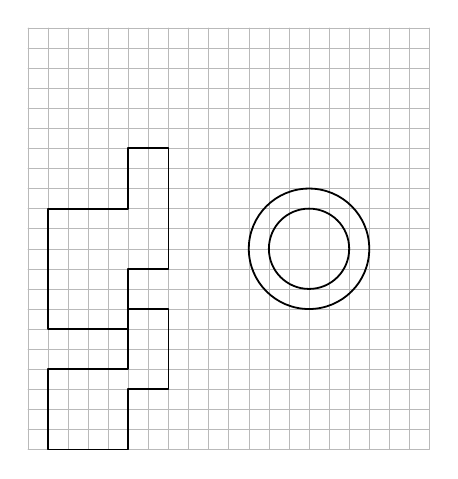
\begin{tikzpicture}[x=2.55mm,y=2.55mm,line cap=round,line join=round]
  % 细灰色方格与题给粗实线分层；原图没有虚线。
  \draw[step=1,gray!55,line width=.18pt] (0,-3) grid (20,18);
  % 左上投影。
  \draw[line width=.65pt] (1,9)--(5,9)--(5,12)--(7,12)--(7,6)--(5,6)--(5,3)--(1,3)--cycle;
  % 左下投影。
  \draw[line width=.65pt] (1,1)--(5,1)--(5,4)--(7,4)--(7,0)--(5,0)--(5,-3)--(1,-3)--cycle;
  % 右上投影：两个同心圆。
  \draw[line width=.65pt] (14,7) circle[radius=3];
  \draw[line width=.65pt] (14,7) circle[radius=2];
\end{tikzpicture}
